\chapter{Determining Structural Correspondences}\label{background2}
In order to construct a structural generalization describing the commonalities and differences between ASTs of two given logged methods (LMs), we first need to find structural correspondences between their nodes. My approach to determining correspondences proceeds in three steps: first, computing similarity between AST nodes (Section~\ref{jigsaw-similarity}); second, determining potential structural correspondences between AST nodes (Section~\ref{jigsaw-corr}); third, constructing an extended form of ASTs, called AUASTs (anti-unifier ASTs) to allow the creation of an anti-unified structure (Section~\ref{jigsaw-corr}) in a later phase. To evaluate my approach, I implemented it as an Eclipse plug-in, named the correspondence tool, which is built atop Jigsaw. Then I conducted an experimental study to validate its effectiveness for my application. Section~\ref{jigsaw-assessment} describes my experimental setup, present my study, and discuss the results.
% first, the ASTs of Java methods are extracted from source code;

To develop the correspondence tool, I first needed a concrete framework for constructing and manipulating ASTs. The Eclipse integrated development environment provides such a framework in its Java Development Tools (JDT) component (as explained in Section~\ref{JDT-impl}). I also utilized Jigsaw \cite{2008:fse:cottrell}, which is an existing framework for creating structural correspondence connections among ASTs based on the structural similarity between their nodes (Section~\ref{Jigsaw-impl}). I then constructed the AUAST structure to allow the insertion of variables in place of any nodes. I built atop this work in order to create anti-unifiers.
%we or I???
% and a comparison of our tool with Jigsaw (Section~\ref{comparison-Jigsaw}).
%jEdit v4.2 pre 15 (2004)


%\subsection{Extracting the ASTs of LMs}\label{Jigsaw_usage}
%In order to describe the structure of Java methods that make use of logging calls in a program, we need to extract their ASTs (as described in Section~\ref{AST}).



\section{Computing similarity}  \label{jigsaw-similarity}
To compute similarity between AST nodes, I re-used a function developed by \citet{2008:fse:cottrell} that relies on syntactic similarity along simple knowledge of semantic equivalences supported by a program language specifications. It returns a value in $[0, 1]$ where zero indicates complete lack of similarity and one indicates perfect similarity. In general, this function returns a value above zero if the compared nodes are of identical type, and thus it returns a similarity of 0 for nodes of different types.
However, it uses several heuristics to improve the accuracy of similarity measurement by defining an arbitrary value for the nodes that are syntactically different but are semantically relevant. For example, the similarity between names of AST nodes is measured using a normalized computation based on the length of the longest common substring. The comparison of the \code{int} and \code{long} nodes is another example, where an arbitrary value of 0.5 is defined as the similarity, since they are not of syntactically identical types but have semantic equivalences. The function also detects the structural correspondence between \code{for}-, \code{enhanced-for}-, \code{while}-, and \code{do}-loop statements; and \code{if} and \code{switch} conditional statements.
%bradly citation ????

\citet{2008:fse:cottrell} computed the similarity between non-leaf nodes not only based on the node types, but also pairwise similarities of their children nodes, as described via the \func{Non-Leaf-Node-Similarity} algorithm. In this algorithm, the children of the subtrees $\id{astA}$ and $\id{astB}$ are compared exhaustively in a pairwise manner (Lines~1--10). For each child node of the subtree $\id{astA}$, the highest similarity with any child node of the subtree $\id{astB}$ is determined (Lines~4--9) . All these maximum similarities are summed up and divided by the size of the largest subtree (Lines~11--12).

% should be modified???
\begin{algorithm}
  \caption{\func{Non-Leaf-Node-Similarity}($\id{astA}$,$\id{astB}$) computes the similarity between two non-leaf nodes.}
  \label{computeMatches}
  \begin{algorithmic}[1]
  \Non-Leaf-Node-Similarity
  	 %  \State{$ \func{Determine-Best-Correspondence}(\id{auastA}, \id{auastB})$}
  	  % \EndIf
         \State $\id{sum} \gets 0$
      \For {$\id{childA} \in \id{children}[\id{astA}]$}
		\State $\id{max} \gets 0$
     		
		\For {$\id{childB} \in \id{children}[\id{astB}]$}	
 			\State $\id{sim} \gets  \func{Similarity}(childA,childB)$	
 		\If {$\id{sim} > \id{max}$ }	
 		\State $\id{max} \gets \id{sim}$	
		\EndIf 		
 \EndFor 	
	  \EndFor 	
	 	
	    \State $\id{sum} \gets  \id{sum} +  \id{max}$
	
%       \EndFor 	
	\Return $\id{sum} / \id{max}{|\id{auastA}| + |\id{auastB}|}$

  \end{algorithmic}
\end{algorithm}



\section{Determining potential correspondences}  \label{jigsaw-corr}

%The goal of this phase is to determine potential correspondences between AST nodes, for use in the generalization phase.
The similarity function can be used to determine potential structural correspondences amongst nodes of two given ASTs. To find correspondences, I used an algorithm proposed by \citet{2008:fse:cottrell} that generates an augmented form of AST, called \emph{correspondence AST} (CAST), where each node holds a list of candidate correspondence connections, each implicitly representing an anti-unifier. The \func{Determine-Potential-Correspondences} algorithm computes the similarity for all pairs of nodes in the two ASTs (Lines~1--3). If similarity value for a pair is above zero, a correspondence connection will be created and added to the list of correspondence connections of the two corresponding nodes (Lines~4--8). As an example, Figure~\ref{fig:meth-ast-1} shows candidate structural correspondence connections created via the \func{Determine-Potential-Correspondences} algorithm on ASTs of Examples 1 and 2.


\begin{algorithm}
  \caption{\func{Determine-Potential-Correspondences}($\id{astA}$,$\id{astB}$) determines the candidate correspondence connections between the nodes of $\id{astA}$ and $\id{astB}$.}
  \label{computeMatches}
  \begin{algorithmic}[1]
  \DeterminePotentialCorrespondences
      \For {$\id{nodeA} \in \id{astA}$}
 		%\State $\id{corrsA} \gets \cons{Null}$	
		
		\For {$\id{nodeB} \in \id{astB}$}
		\State $\id{sim} \gets \func{Similarity}(nodeA,nodeB)$	
 			\If {$sim > 0$}	
 		\State $\id{corr} \gets \func{create-correspondence-connection}(\id{nodeA},\id{nodeB},\id{sim})$	
 \State $\func{Append}(\id{corrs}[\id{nodeA}],corr)$	
 \State $\func{Append}(\id{corrs}[\id{nodeB}],corr)$
 		\EndIf 		
 \EndFor 	
	  \EndFor 	
	
  \end{algorithmic}
\end{algorithm}



\begin{figure} [H]  \centering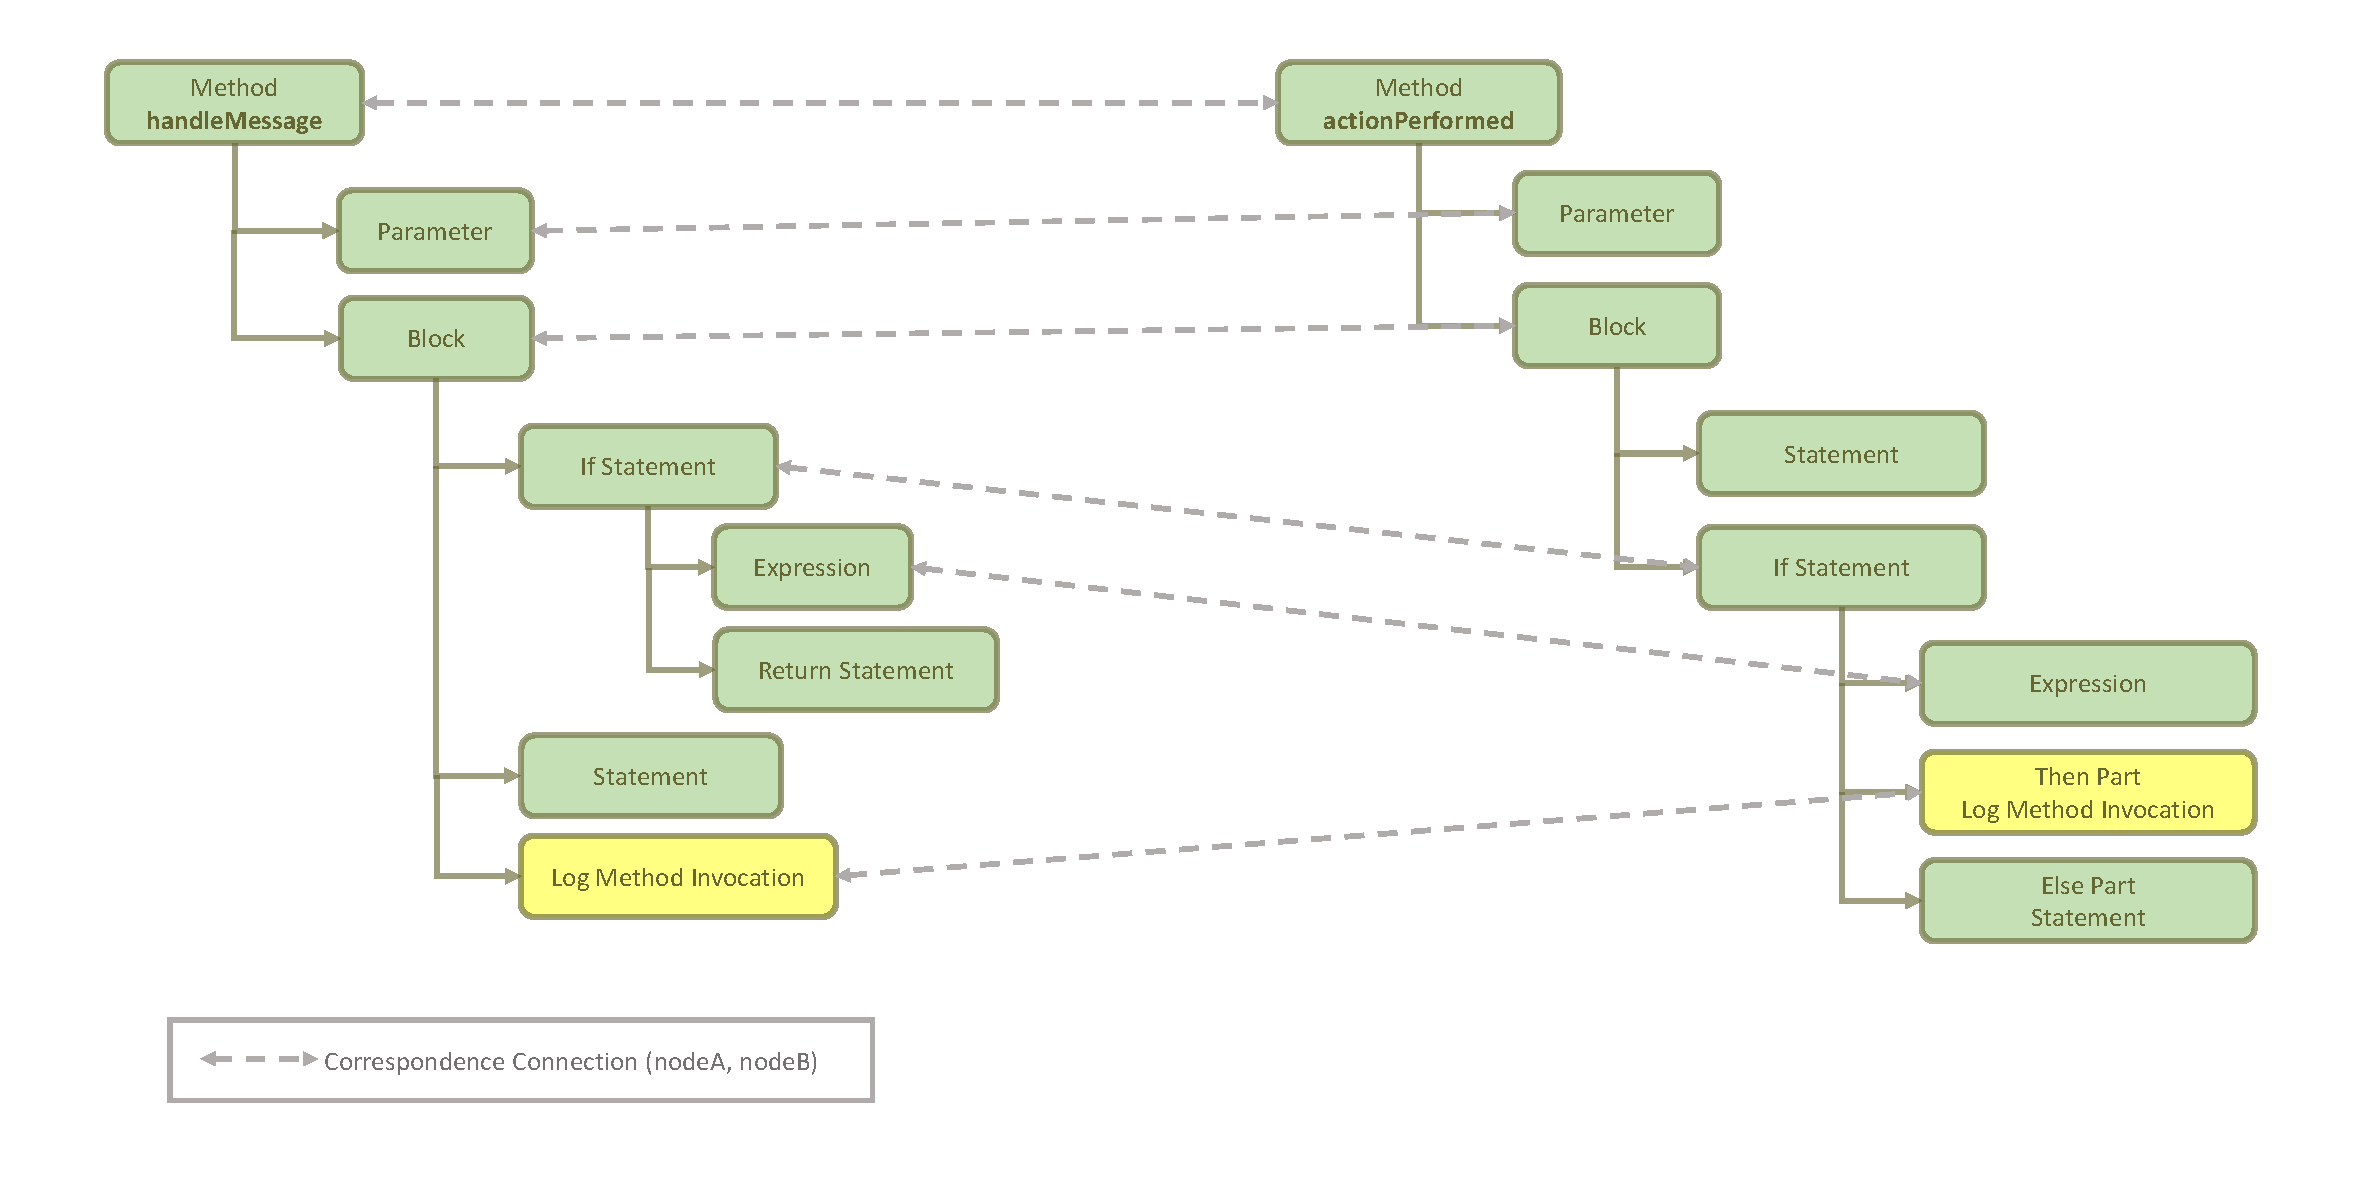
\includegraphics [width = \textwidth]{Drawing4/FirstCorr.pdf}
  \caption[Simple CAST structure of the examples in Figures~\ref{ch3-ex1} and~\ref{ch3-ex2}.]{Simple CAST structure of the examples in Figures~\ref{ch3-ex1} and~\ref{ch3-ex2}. The links between CAST nodes indicate structural correspondence connections created using the \func{Determine-Potential-Correspondences} algorithm.}
  \label{fig:meth-ast-1}
\end{figure}

\section{Constructing the AUAST}  \label{jigsaw-corr}
%\RW{This is a concrete implementation, not a generic idea, at least not the way it is described. I strongly suggest that you give a generic description of your assumptions about ASTs then relate AUASTs to those, then talk about implementation details.}
%\NZ{I tried to explain the concept.}
%
As described in Section~\ref{HOAUMT}, an anti-unified structure utilizes variables that must be substituted with proper substructures to regain original structures. However, the CAST structure presented by \citet{2008:fse:cottrell} would allow the creation of an anti-unified structure, as it does not contain any variables. Therefore, an extended form of it is required, namely the AUAST (anti-unifier AST), that would allow the insertion of variables in place of any node in the tree structure, including both subtrees and leaves, to indicate variations between the original structures.
%namely?

To provide an example to demonstrate this structure, the anti-unified AUAST constructed from the AUASTs of logging calls in Figures~\ref{ch3-ex1} and~\ref{ch3-ex2} is depicted in Figure~\ref{fig:logging-anti}. The structural variables $X$ and $Y$ are used to indicate the structural variations, where the $X$ structural variable refers to two simple names and the $Y$ structural variable refers to two subtrees. The substitutions are defined in Equations~\ref{eq:theta1} and~\ref{eq:theta2}.

% leaf- non leaf refer???

\begin{align}
\Theta_1 = (X \rightarrow \text{ \textsf{\small WARNING}}, Y \rightarrow \text{ \textit{additionExpression}(}\hspace*{3cm}\nonumber\\
\text{\textit{methodCall}(\textit{simpleName}(\textsf{\small getClassName}), \textit{arguments}()),}\nonumber\\
\text{\textit{stringLiteral}(\textsf{\small "should extend ..."}),}\hspace*{4cm}\nonumber\\
\text{\textit{methodCall}(\textit{simpleName}(\textsf{\small handleMessage}), \textit{arguments}()))})\hspace*{-1em}\label{eq:theta1}
\end{align}

\begin{align}
\Theta_2 = (X \rightarrow \text{ \textsf{\small ERROR}}, Y \rightarrow \text{ \textit{additionExpression}(}\hspace*{3cm}\nonumber\\
\text{\textit{stringLiteral}(\textsf{\small "Unknown action: "})},\nonumber\\
\text{ \textit{simpleName}(\textsf{\small actionName}))})\hspace*{-1cm}\label{eq:theta2}
\end{align}

%\item it can be mapped to our recursive definition of a term, where AST nodes and simple values may be viewed as function-symbols and constants, respectively

\begin{figure}[p]
\begin{small}
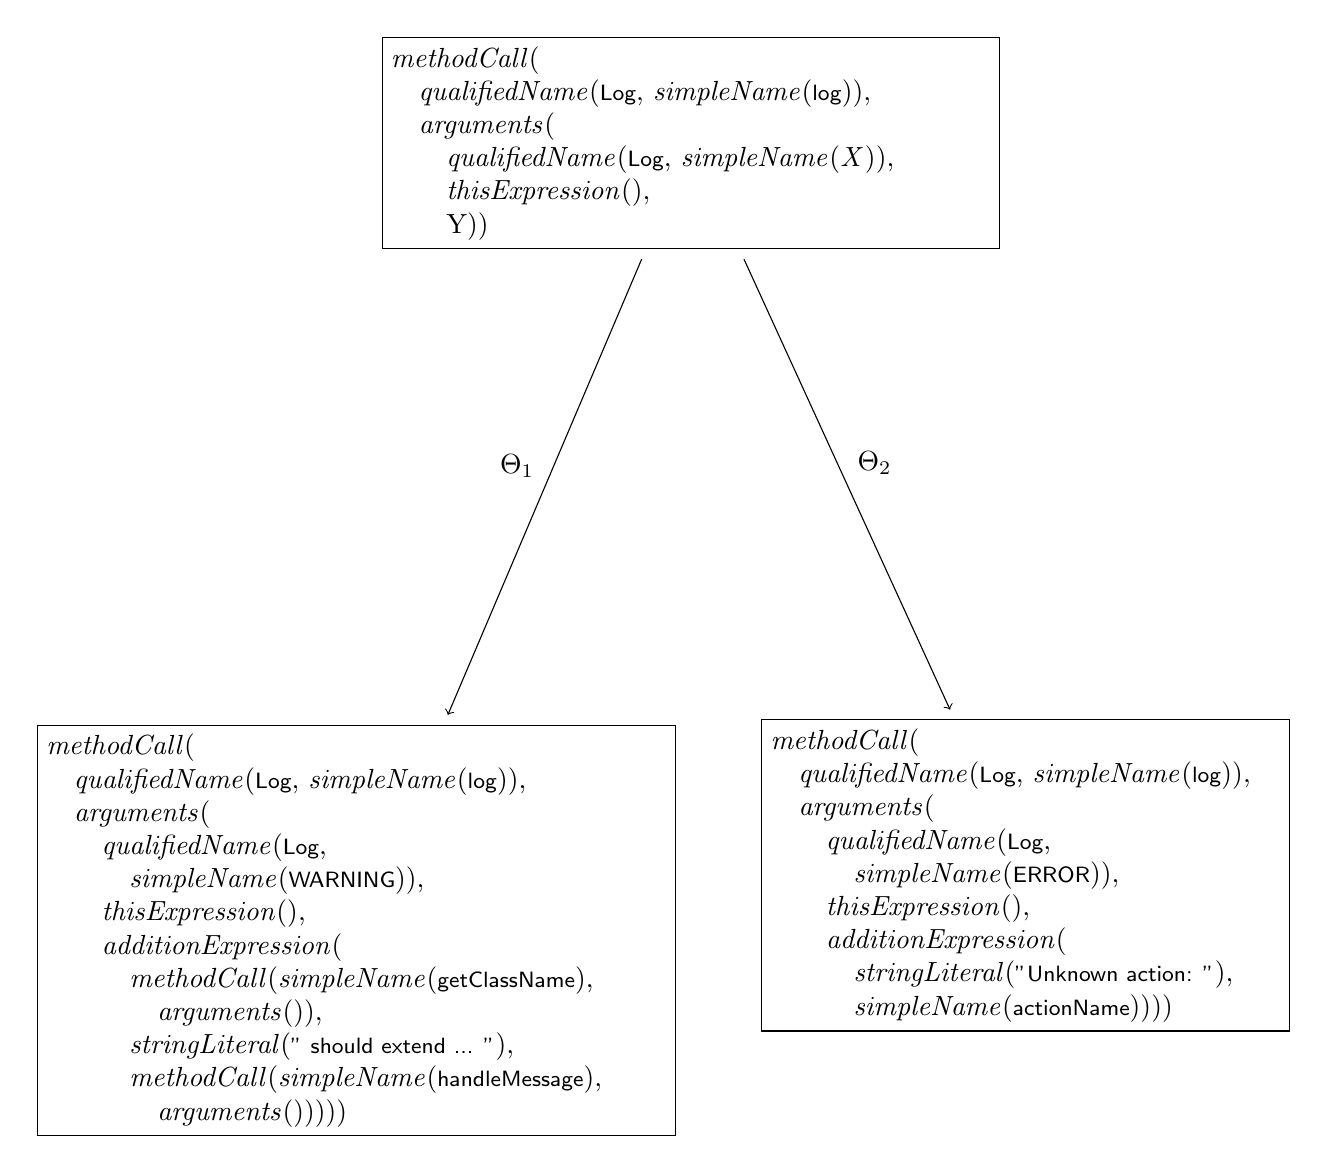
\begin{tikzpicture}
\node(a) at (4.25,10) {%
\fbox{\parbox[b][][b]{3in}{%
\text{\textit{methodCall}(}\\
\text{\hspace*{1em}\textit{qualifiedName}(\textsf{\footnotesize Log}, \textit{simpleName}(\textsf{\footnotesize log})),}\\
\text{\hspace*{1em}\textit{arguments}(}\\
\text{\hspace*{2em}\textit{qualifiedName}(\textsf{\footnotesize Log}, \textit{simpleName}(\textit{X})),}\\
\text{\hspace*{2em}\textit{thisExpression}(),}\\
\text{\hspace*{2em}Y))}}}%
};
\node(b) at (0,0) {%
\fbox{\parbox[t][][b]{3.1in}{%
\text{\textit{methodCall}(}\\
\text{\hspace*{1em}\textit{qualifiedName}(\textsf{\footnotesize Log}, \textit{simpleName}(\textsf{\footnotesize log})),}\\
\text{\hspace*{1em}\textit{arguments}(}\\
\text{\hspace*{2em}\textit{qualifiedName}(\textsf{\footnotesize Log},}\\ \text{\hspace*{3em}\mbox{\textit{simpleName}(\textsf{\footnotesize WARNING})}),}\\
\text{\hspace*{2em}\textit{thisExpression}(),}\\
\text{\hspace*{2em}\textit{additionExpression}(}\\
\text{\hspace*{3em}\textit{methodCall}(\textit{simpleName}(\textsf{\footnotesize getClassName}),}\\ \text{\hspace*{4em}\textit{arguments}()),}\\
\text{\hspace*{3em}\textit{stringLiteral}(\textsf{\footnotesize " should extend ... "}),}\\
\text{\hspace*{3em}\textit{methodCall}(\textit{simpleName}(\textsf{\footnotesize handleMessage}),}\\ \text{\hspace*{4em}\textit{arguments}()))))}}}%
};
\node(c) at (8.5,0.7) {%
\fbox{\parbox[t][][b]{2.55in}{%
\text{\textit{methodCall}(}\\
\text{\hspace*{1em}\textit{qualifiedName}(\textsf{\footnotesize Log}, \textit{simpleName}(\textsf{\footnotesize log})),}\\
\text{\hspace*{1em}\textit{arguments}(}\\
\text{\hspace*{2em}\textit{qualifiedName}(\textsf{\footnotesize Log},}\\ \text{\hspace*{3em}\mbox{\textit{simpleName}(\textsf{\footnotesize ERROR})}),}\\
\text{\hspace*{2em}\textit{thisExpression}(),}\\
\text{\hspace*{2em}\textit{additionExpression}(}\\
\text{\hspace*{3em}\textit{stringLiteral}(\textsf{\footnotesize "Unknown action: "}),}\\
\text{\hspace*{3em}\textit{simpleName}(\textsf{\footnotesize actionName}))))}}}%
};

\draw[->](a) -- (b) node[pos=0.5,above]{$\Theta_1\qquad$};
\draw[->](a) -- (c) node[pos=0.5,above]{$\qquad\Theta_2$};
\end{tikzpicture}
\end{small}
\caption{Anti-unification of the AUASTs of the logging calls in Examples 1 and 2.\label{fig:logging-anti}}
\end{figure}






%\begin{align}
%\Theta_1 = (W &\rightarrow \text{ \textsf{\small WARNING}},\nonumber\\
%X &\rightarrow \text{ \textit{methodCall}(\textit{simpleName}(\textsf{\small getClassName}), \textit{arguments}())},\nonumber\\
%Y &\rightarrow \text{ \textsf{\small "should extend EditPlugin not EBPlugin since it has an empty "}},\nonumber\\
%Z &\rightarrow \text{ \textit{methodCall}(\textit{simpleName}(\textsf{\small handleMessage}), \textit{arguments}())})\label{eq:theta1}\\
%\Theta_2 = (W &\rightarrow \text{ \textsf{\small ERROR}},\nonumber\\
%X &\rightarrow \text{ \NIL{}},\nonumber\\
%Y &\rightarrow \text{ \textsf{\small "Unknown action: "}},\nonumber\\
%Z &\rightarrow \text{ \textit{simpleName}(\textsf{\small actionName})})\label{eq:theta2}
%\end{align}
%
%%\item it can be mapped to our recursive definition of a term, where AST nodes and simple values may be viewed as function-symbols and constants, respectively
%
%\begin{figure}[p]
%\begin{small}
%\begin{tikzpicture}
%\node(a) at (4.25,10) {%
%\fbox{\parbox[b][][b]{3in}{%
%\text{\textit{methodCall}(}\\
%\text{\hspace*{1em}\textit{qualifiedName}(\textsf{\footnotesize Log}, \textit{simpleName}(\textsf{\footnotesize log})),}\\
%\text{\hspace*{1em}\textit{arguments}(}\\
%\text{\hspace*{2em}\textit{qualifiedName}(\textsf{\footnotesize Log}, \textit{simpleName}(\textit{W})),}\\
%\text{\hspace*{2em}\textit{thisExpression}(),}\\
%\text{\hspace*{2em}\textit{additionExpression}(\textit{X}, \textit{stringLiteral}(\textit{Y}), \textit{Z})))}}}%
%};
%\node(b) at (0,0) {%
%\fbox{\parbox[t][][b]{3.1in}{%
%\text{\textit{methodCall}(}\\
%\text{\hspace*{1em}\textit{qualifiedName}(\textsf{\footnotesize Log}, \textit{simpleName}(\textsf{\footnotesize log})),}\\
%\text{\hspace*{1em}\textit{arguments}(}\\
%\text{\hspace*{2em}\textit{qualifiedName}(\textsf{\footnotesize Log},}\\ \text{\hspace*{3em}\mbox{\textit{simpleName}(\textsf{\footnotesize WARNING})}),}\\
%\text{\hspace*{2em}\textit{thisExpression}(),}\\
%\text{\hspace*{2em}\textit{additionExpression}(}\\
%\text{\hspace*{3em}\textit{methodCall}(\textit{simpleName}(\textsf{\footnotesize getClassName}),}\\ \text{\hspace*{4em}\textit{arguments}()),}\\
%\text{\hspace*{3em}\textit{stringLiteral}(\textsf{\footnotesize " should extend ... "}),}\\
%\text{\hspace*{3em}\textit{methodCall}(\textit{simpleName}(\textsf{\footnotesize handleMessage}),}\\ \text{\hspace*{4em}\textit{arguments}()))))}}}%
%};
%\node(c) at (8.5,0.7) {%
%\fbox{\parbox[t][][b]{2.55in}{%
%\text{\textit{methodCall}(}\\
%\text{\hspace*{1em}\textit{qualifiedName}(\textsf{\footnotesize Log}, \textit{simpleName}(\textsf{\footnotesize log})),}\\
%\text{\hspace*{1em}\textit{arguments}(}\\
%\text{\hspace*{2em}\textit{qualifiedName}(\textsf{\footnotesize Log},}\\ \text{\hspace*{3em}\mbox{\textit{simpleName}(\textsf{\footnotesize ERROR})}),}\\
%\text{\hspace*{2em}\textit{thisExpression}(),}\\
%\text{\hspace*{2em}\textit{additionExpression}(}\\
%\text{\hspace*{3em}\textit{stringLiteral}(\textsf{\footnotesize "Unknown action: "}),}\\
%\text{\hspace*{3em}\textit{simpleName}(\textsf{\footnotesize actionName}))))}}}%
%};
%
%\draw[->](a) -- (b) node[pos=0.5,above]{$\Theta_1\qquad$};
%\draw[->](a) -- (c) node[pos=0.5,above]{$\qquad\Theta_2$};
%\end{tikzpicture}
%\end{small}
%\caption{The anti-unification of the AUASTs of the logging calls in Examples 1 and 2.\label{fig:logging-anti}}
%\end{figure}
%%The AUASTs of log Method Invocation nodes from the Java classes in Figure~\ref{ch3-ex1} and Figure~\ref{ch3-ex2}.

%Applying higher-order anti-unification on AUAST structures could help to construct a structural generalization by maintaining the common pieces and abstracting the differences away using variables. However, it is not comprehensive enough to solve our problem as it does not consider background knowledge about AST structures, such as syntactically different but semantically relevant structures, missing structures, and different ordering of arguments. In the following section, we will look at an extension of anti-unification, higher-order anti-unification modulo theories, and how it can sufficiently address the limitations of anti-unification in our context.

%We provide an example to demonstrate the AUAST structure, which is limited to log method invocation subtrees of the sample Java classes shown in Figure~\ref{fig:constructAUast}. The log method invocation nodes both contains \texttt{EXPRESSION}, \texttt{ARGUEMENTS}, and \texttt{NAME} structural properties which are made up of \texttt{\bold{Log}}, \texttt{\bold{Log}}, \texttt{\bold{WARNING}} simple values for the AUAST1 and  \texttt{\bold{Log}}, \texttt{\bold{Log}}, \texttt{\bold{ERROR}} simple values for the AUAST2, respectively. The structural representation of the AUASTs as defined in Section~\ref{back-str} is \texttt{EXPRESSION[EXPRESSION[IDENTIFIER[\bold{Log}]], ARGUMENTS[QUALIFIER[IDENT\\IFIER[\bold{Log}]], NAME[IDENTIFIER[\bold{WARNING}]]}for the AUAST1 and \texttt{EXPRESSION[EX\\PRESSION[IDENTIFIER[\bold{Log}]], ARGUMENTS[QUALIFIER[IDENTIFIER[\bold{Log}]], \\NAME[IDENTIFIER[\bold{ERROR}]]} for the AUAST2, where the words capitalized represents subtrees and the words shown in bold represents leaves of the tree structure.

%\begin{figure} [H]
 % \centering\includegraphics [width = \textwidth, height = 0.4\textheight]
 % {Drawing4/structure1.pdf}
 % \caption{The AUASTs of log Method Invocation nodes from the Java classes in Figure~\ref{ch3-ex1} and Figure~\ref{ch3-ex2}.}
 % \label{fig:constructAUast}
%\end{figure}


%to construct structural generalizations?




\section{The correspondence tool}\label{corr-tool}

%I implemented a plug-in to the Eclipse integrated development environment (IDE), which uses the \name{JDT} framework to extract ASTs of a pair of LMs and applies the \name{Jigsaw} framework to generate correspondence connections between AST nodes.

The correspondence tool is a proof-of-concept implementation of the proposed approach to determining potential structural correspondences, which is an Eclipse plug-in that inputs a Java program, extracts ASTs of logged methods in it using the Eclipse JDT framework, applies a part of the implementation of Jigsaw to identify structural correspondences between ASTs in a pairwise manner and reuses the Jigsaw similarity function to measure the similarity between nodes involved in each correspondence connection. It also creates an extended form of CAST, called AUAST, which  addresses the limitations of the CAST structure to constructing an anti-unifier by adding the following structural properties:
%namely?

\begin{itemize} [leftmargin=.5in]
\item \textit{Simple structural variable Properties}: an extension of simple structural properties referring to two simple values to allow the insertion of variables in place of leaves.
\end{itemize}
\begin{itemize} [leftmargin=.5in]
\item \textit{Child structural variable properties}: an extension of child structural properties referring to two child AST nodes to allow the insertion of variables in place of subtrees.
\end{itemize}

%%change???





\section{Evaluation}\label{jigsaw-assessment}
%\section{An Assessment of the Correspondence tool}\label{jigsaw-assessment}
%\section{The Correspondence tool} \label{correspondenceTool}
%
%\RW{Describe here the procedure you used to select the examples, etc., how you tested Jigsaw, and what your findings were. At some point, you complained that Cottrell had not done something right ... do you have any evidence to demonstrate it?  How does this affect your work?  Such points can go in a discussion section towards the end of this chapter if they don't fit otherwise.  Full details of examples can go in an appendix; here, just describe enough so people can get the point.}
%
%\NZ{I think this experiment is not much about evaluating Jigsaw (The evaluation was conducted by Cottrell), but it is more about understanding what Jigsaw does and how to use it for my application . What I have mentioned was about detecting relevance links which is not related to my work. During my development, I added some statements to Jigsaw for the cases that was not covered in his work completely (e.g, Jigsaw did not detect the correspondence between inner type declarations of two nested type declarations when comparing the two upper type declarations }
%
%
To evaluate the proposed approach and the tool support, I conducted an experiment on a set of LMs extracted from a real-world software system to assess how Jigsaw could effectively help us determine potential correspondences between AST nodes and measure similarity between them.

%Jigsaw or correspondence???


%chapter{Experimental Studies}  \label{studies}
%To evaluate our approach, we have implemented a tool, and conducted three empirical studies on a set of LMs extracted from a real-world software system. In this section, we describe our experimental setup, present our studies, and discuss the results.



%the correspondence tool as
%\subsubsection{Experimental Setup}  \label{study1_setup}
\subsection{Setup}  \label{study1_setup}
%Our tool is a plug-in to the Eclipse integrated development environment (IDE) that implements our algorithm. The tool consists of three main components: a correspondence tool, an antiunifier-building tool, and a clustering tool. The correspondence tool inputs a pair of LMs, uses the Jigsaw framework to determine potential correspondences between their AST nodes, and outputs the generated CASTs and the Jigsaw similarity between them. The antiunifier-building tool inputs a pair of LMs, applies our anti-unification algorithm to construct an anti-unifier with a special attention to logging calls, and outputs the detailed view of anti-unifier and similarity measure (as described in Section~\ref{meth-antiUnifier}). The clustering tool inputs a set of LMs, applies a hierarchical clustering algorithm to classify them based on the similarity measurement, and outputs the detailed view of the generated anti-unifier for each cluster (as described in Section~\ref{meth-clustering}).
% figure of architecture?

As a subject for our study, we used \name{jEdit}, a programmer's text editor tool written in Java programming language. We chose this subject because it is a real program that has been used constantly by many developers, and it employs real usage of logging calls. Our tool extracts all LMs within the source code of this program. However, a subset of them was selected containing 9 LMs that showed varying levels of similarity on manual examination, and it has been used as a test suite throughout this study (see Table~\ref{table:ljms}). The \code{org.gjt.sp.jedit.EditBus.send(...)} method contains two logging calls. To handle this case we split it into two cases: case 3 contained the first logging call while the second one was removed; case 4 contained only the second logging call. We will describe our approach for LMs containing multiple logging calls in details in Section~\ref{meth-multipleLogs}. The last three LMs were manually modified by adding some statements for the sake of dealing with important cases that we otherwise would have missed testing. Case 8 simulates the addition of an \code{if}-statement that formed a nested \code{if}-statement enclosing a logging call. Cases 9 and 10 simulate the addition of statements to improve the test coverage.


\begin{figure} [H]
  \centering
  \begin{tabular}{clc}
    \toprule
    Case & Logged Java methods & Size (LOC)\\
    \midrule
    1& \code{PluginJAR.generateCache()} &104\\
    2& \code{MiscUtilities.isSupportedEncoding(...)} &9\\
    3& \code{EditBus.send(...)} &14\\
    4& \code{EditBus.send(...)}* &14\\
    5& \code{EditAction.Wrapper.actionPerformed(...)} &5\\
    6& \code{EBPlugin.handleMessage(...)} &6\\
    7& \code{BufferHistory.RecentHandler.doctypeDecl(...)} &3\\
    8& \code{JARClassLoader.loadClass(...)} &32\\
    9& \code{VFS.DirectoryEntry.RootsEntry.rootEntry(...)} &36\\
    10& \code{ServiceManager.loadServices(...)} &20\\
    \bottomrule
  \end{tabular}
  \caption[Logged Java methods used as our test suite.]{Logged Java methods used as our test suite; all are contained in the \protect\name{org.gjt.sp.jedit} package with the exception of case 9 that is in the \protect\name{org.gjt.sp.jedit.io} package.}
  \label{table:ljms}
\end{figure}


%\subsubsection{Setup}  \label{study1-setup}
Our tool was used to compare LMs of our test suite in a pairwise manner (55 test cases in total, including self-comparisons) and to produce the CASTs of each pair. The Jigsaw similarity was also measured for each of these test cases.
We examined the generated CASTs of these test cases and selected a subset of 4 cases with various levels of correspondences as depicted in the Table~\ref{jigsaw_4_test_cases}. Case 1 contains the comparison of a Java element with itself. Case 2 contains the comparison of two Java elements that are both syntactically and semantically dissimilar.  Case 3 contains the correspondence between two Java elements that are syntactically dissimilar but are semantically relevant. Case 4 contains the comparison of a logging call with another Java element that is not logging call but is syntactically relevant.

\subsection{Results}  \label{study1-results}
The results of the pairwise comparison between LMs of the test suite is visualized in Figure~\ref{fig:jigsaw_graph}. As it is shown, the Jigsaw similarity for all self-comparisons is 1, while  the level of Jigsaw similarity is different for pairs containing distinct LMs as our manual examination.

\begin{figure} [H]
  \centering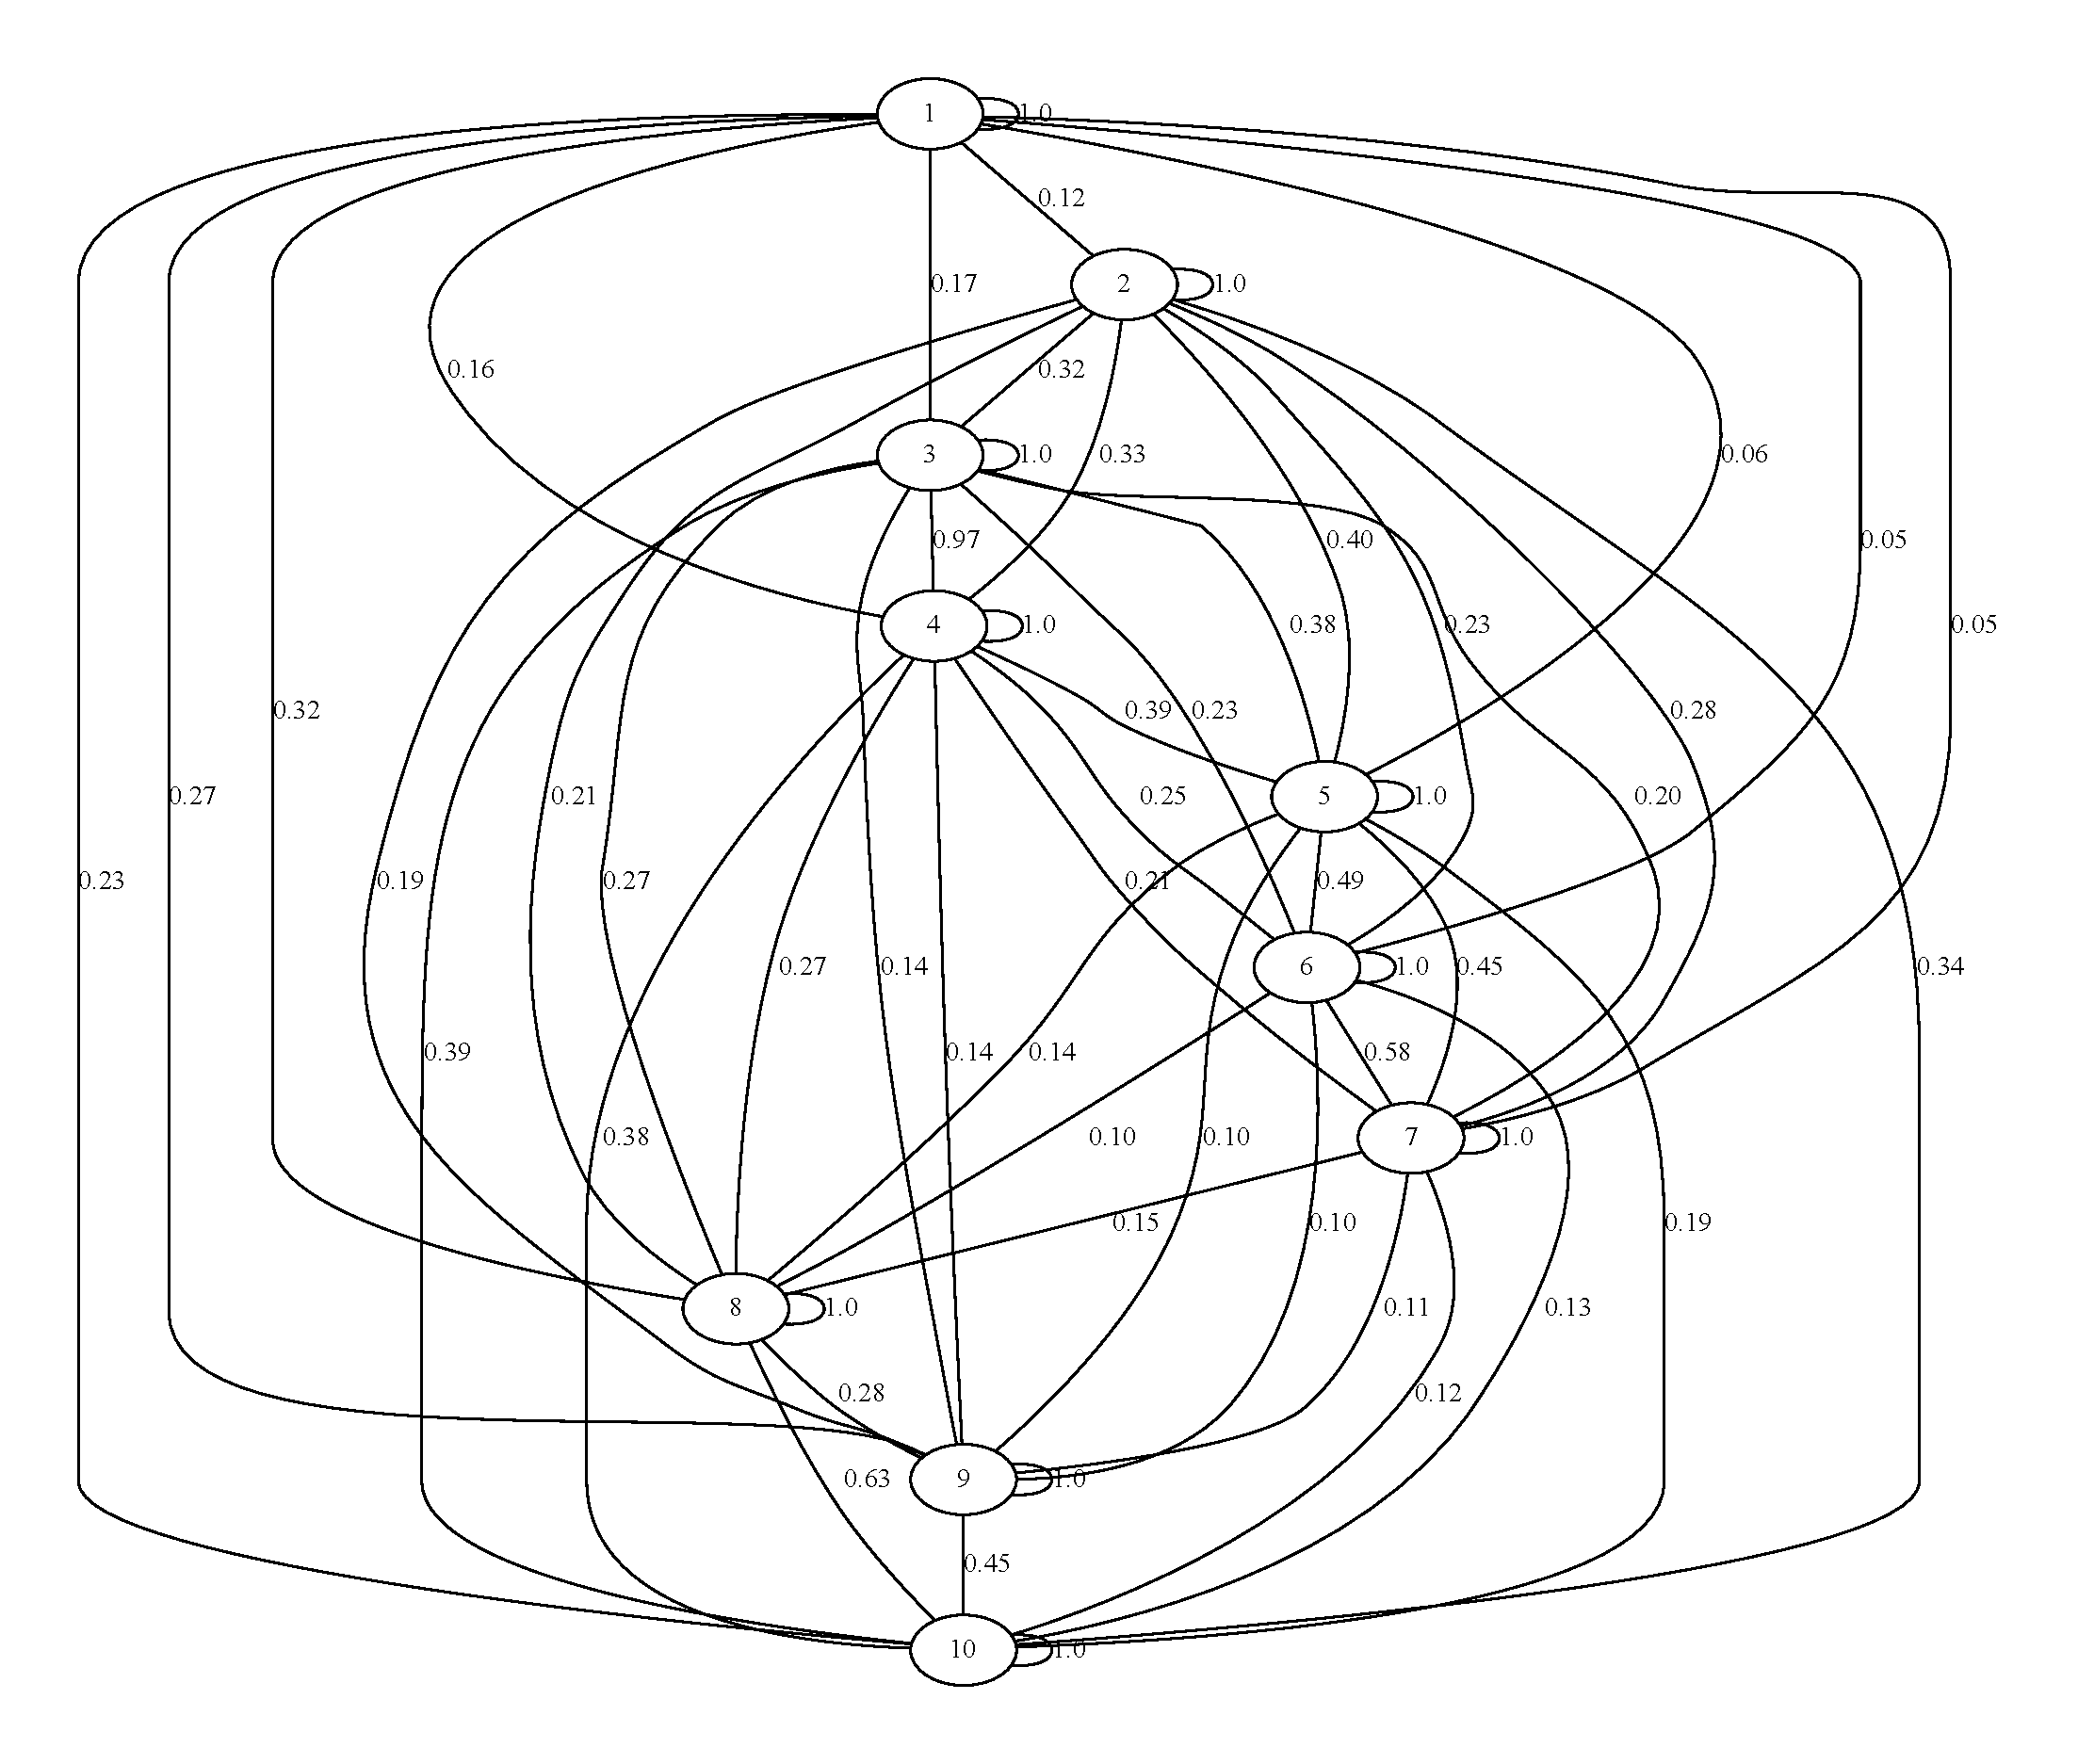
\includegraphics [width = \textwidth]{graphviz/jigsaw.pdf}
  \caption{A similarity graph representing pairwise Jigsaw similarities between LMs shown in Table~\ref{table:ljms}.}
  \label{fig:jigsaw_graph}
\end{figure}


The analysis of the 4 cases is shown in Table~\ref{jigsaw_4_test_cases}. Case 1 shows that a Java element that is compared with itself has a Jigsaw similarity of 1. Case 2 indicates that no correspondence connection is created when a Java element is compared with another Java element that is utterly dissimilar. Case 3 indicates that the similarity between a \code{for}-statement and a \code{while}-statement is non-zero, and that Jigsaw is able to detect semantic correspondences between Java elements. Case 4 shows that a logging call has non-zero similarity with another Java element that is not a logging call but is syntactically relevant. This case will be handled via the removal of this kind of correspondence connection, as will be described in Section~\ref{meth-constraints}. \RW{Section???}

\begin{figure}
  \centering
  \begin{tabular}{clc}
    \toprule
    \shortstack{Test\\case} & Java source code fragment & \shortstack{Jigsaw\\similarity}\\
    \midrule

    \multirow{2}{*}{{1}}&\code{Log.log(Log.WARNING,this,"Unknown action: " + actionName);}& \multirow{2}{*}{1}\\
    
                         &\code{Log.log(Log.WARNING,this,"Unknown action: " + actionName);}\\
    \midrule

       \multirow{2}{*}{2}&\code{return entry;}& \multirow{2}{*}{0}\\
       &\code{int i=0;}\\
    \midrule


 \multirow{2}{*}{3}&
 \code/for (int i=0; i < comps.length; i++) {...}/&\multirow{2}{*}{\RW{???}}\\


      &
\code/while (entries.hasMoreElements())  { ...}/
      \\
    \midrule

    \multirow{2}{*}{4}&\code{Log.log(Log.WARNING,this,"Unknown action: " + actionName);}& \multirow{2}{*}{0.33}\\
      &\code{EditBus.removeFromBus(this);}\\
    \bottomrule

  \end{tabular}
  \caption{Results from examining the Jigsaw similarity for 4 sample Java source code fragment pairs.}
  \label{jigsaw_4_test_cases}
\end{figure}

%\section{Comparison with the Jigsaw tool}  \label{comparison-Jigsaw}


\subsection{discussion}  \label{study2-results}
Though the results of this experiment validates Jigsaw's functionality in determining potential correspondences between ASTs nodes, it does not suffice to construct structural generalizations needed in my context. As the problem of this study is different, I should build atop this tool to address the following issues:

\begin{itemize} [leftmargin=.5in]
\item The CAST structure does not allow the creation of an anti-unified structure, as it does not allow the insertion of variables in place of any nodes in the tree structure.
\item The Jigsaw tool does not create a detailed view of the anti-unifier describing the commonalities and differences between logged Java methods.
\item The Jigsaw tool does not determine the best correspondences with special attention to logging calls to construct an approximation of the best anti-unifier for my problem.
\item The Jigsaw similarity function does not measure the similarity among the usage of logging calls in Java methods.
% To address these issues, I have developed a greedy selection algorithm to approximate the best anti-unifier for our problem by determining the best correspondence for each node.
\end{itemize}

In the following chapter, I will discuss my approach to construct structural generalization and its implementation by means of the higher-order anti-unification modulo theories.

\section{Summary}  \label{summary}
We described Eclipse JDT as a concrete framework that can be used  to manipulate ASTs of a source code written in the Java programming language. We also introduced Jigsaw, an existing framework for determining structural correspondences between AST nodes and measuring similarity between them. Furthermore, we assess the Jigsaw functionality to address our problem through an empirical study on a set of LMs selected from a real- world software system.





%In this chapter, we described anti-unification as a technique to construct a common generalization of two given terms. We have also introduced an extended form of anti-unification, which is called higher-order anti-unification modulo theories, where a set of equivalence equations can be applied on higher-order extended structures to incorporate background knowledge. In addition, we provided a brief description of AST that maps Java source code in a tree structure form, and why an extended form of it, named AUAST, is required to create higher-order structures specific to our problem context. Finally, we discuss the Jigsaw framework and how it could assist us in determining the potential structural correspondences. 